The first approach has been to analyze some metrics internal to the database.

These metrics are automatically managed by the database itself and show a huge variety of information about the current configuration of the database.

\paragraph{Dynamic Management Views}
    In SQL Server, Dynamic Management Views (\textit{DMVs}) are system views which return server state information useful for monitoring the health of a server instance, diagnosing problems and tuning performance.
    
    The amount of information shown is huge (several thousands of metrics), but only a few have been useful for the performance analyses I carried out.
    
\paragraph{Other metrics}
    Most metrics are related to advanced aspects (e.g. the number of locks performed per second or the number of pages for the whole database) which have proved not to be useful for the performance analyses.
    
    These metrics are indeed used for an in-depth analysis or for advanced tuning of the Data Warehouse.
    
    In my case, however, I wanted to show the difference in query execution times, since it is the most relevant aspect for Axpo employees.

\subsubsection{Metrics Analyzed}
    One of the most important metric analyzed is the execution time of each query submitted to the database.
    
    This value can be retrieved by querying the DMV \texttt{sys.dm\_exec\_query\_stats} \cite{bib:tests:perf:dmv_doc}.
    
    A lot of information are available, such as:
    \begin{itemize}
        \item The query itself.
        \item The execution plan chosen for the query.
        \item How many times the query has been executed.
        \item Execution time.
        \item Physical / Logical reads performed.
        \item Physical / Logical writes performed.
        \item Time used to compile the execution plan.
        \item Memory used to compile the execution plan.
        \item Degree of parallelism (\textit{DOP}).
    \end{itemize}
    
    The only information I decided to analyze is the execution time, since the other were too much specific and low-level.
        
    \paragraph{Values available}
        There are four different values related to execution time:
            \begin{itemize}
                \item Last elapsed time.
                \item Total elapsed time.
                \item Last worker time.
                \item Total worker time.
            \end{itemize}
            
        The first two refer to the total time used for executing the query, while the other are specific to CPU usage.
        
        Both these values are important, since we can compare CPU time to the total elapsed time to understand the impact of locks.
    
    \paragraph{Complications}
        There are however a few complications in this computation.
        
        First of all, if the query has been parallelized (DOP $>$ 1) worker times are aggregated \cite{bib:tests:perf:dmv_time}.
        As a consequence, it is necessary to divide this value by the DOP.
        
        Secondly, all total values need to be divided by the execution count, since we need to compare the execution times independently of how many times a query has been called.
        These values are however stored as integers (without any decimal digits), so they all need to be converted to a decimal type, otherwise we would lose information about decimal digits.
        
        Lastly, values are expressed in microseconds (even though they are accurate up to milliseconds \cite{bib:tests:perf:dmv_doc}).
        These values have been converted to seconds to provide better readability.
        
    \paragraph{Query}
    
        \begin{figure}
            \centering
            \begin{subfigure}{\textwidth}
                \fbox{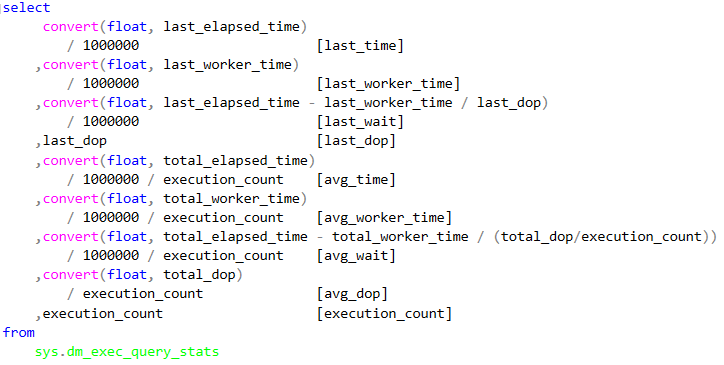
\includegraphics[width=\textwidth]{res/tests/metrics_exec_time_detailed.png}}
                \subcaption{Detailed information.}
                \label{fig:tests:perf:queries:detailed}
            \end{subfigure}
            
            \begin{subfigure}{\textwidth}
                \fbox{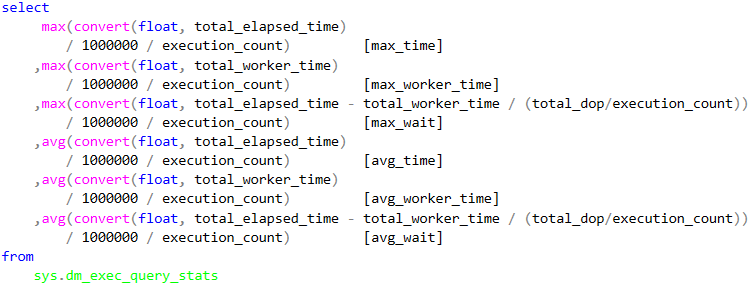
\includegraphics[width=\textwidth]{res/tests/metrics_exec_time_aggregated.png}}
                \subcaption{Average and max metrics.}
                \label{fig:tests:perf:queries:aggregated}
            \end{subfigure}
            
            \caption{Queries used for analyzing query execution times.}
        \end{figure}
        
        Two different queries have been used, as shown in figures \ref{fig:tests:perf:queries:detailed} and \ref{fig:tests:perf:queries:aggregated}.
        The first query produces a detailed output of the execution of each query, while the second shows average and peak execution times across all queries.
        
        \subpar{Aggregate information}
            Aggregate information give a quick but effective overview of the database.
            
            Maximum values show the worst case scenarios, while average values are representative of the database performance.
            We can also understand if there is a problem with locking by comparing elapsed and waiting times.
            If the two values are close, it means that most time was spent waiting.
        
        \subpar{Detailed information}
            Detailed information allow to analyze each query independently.
            
            By ordering the results in descending order, we can easily find how many queries present problems (such as high wait times) or are computationally heavy (which could mean they are not optimized).
            By showing an additional field, called \texttt{sql\_handle}, a unique identifier for that query can be obtained.
            By joining this value with other DMVs, it is possible to perform additional analyses on that specific query.
            
            Last execution times are also shown, since they could differ from average times.
            A large difference can imply there are moments in which the database is under a heavy load and performs poorly.